% auto-generated by benchmarks/src/distributed_spo_gbt/make_paper_tables.py -- regenerate, do not hand-edit

\begin{figure*}[t]
\centering
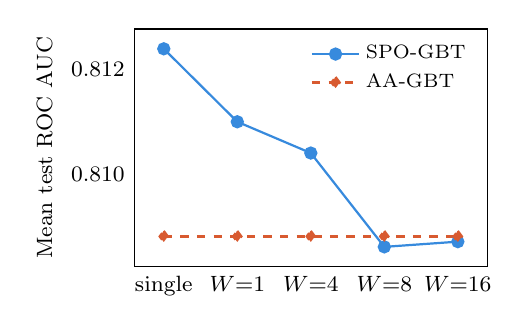
\begin{tikzpicture}
\begin{axis}[width=0.5\textwidth, height=4.6cm, symbolic x coords={Single,1,4,8,16}, xtick=data,
  xticklabels={single,$W{=}1$,$W{=}4$,$W{=}8$,$W{=}16$}, ylabel={Mean test ROC AUC},
  yticklabel style={/pgf/number format/fixed, /pgf/number format/precision=3, /pgf/number format/fixed zerofill},
  tick label style={font=\footnotesize}, label style={font=\footnotesize}, tick style={draw=none},
  legend style={font=\scriptsize, at={(0.98,0.98)}, anchor=north east, draw=none}, legend cell align=left]
\addplot[color={rgb,255:red,55;green,138;blue,221}, mark=*, thick] coordinates {(Single,0.8124) (1,0.8110) (4,0.8104) (8,0.8086) (16,0.8087)};
\addlegendentry{SPO-GBT}
\addplot[color={rgb,255:red,216;green,90;blue,48}, mark=diamond*, thick, dashed] coordinates {(Single,0.8088) (1,0.8088) (4,0.8088) (8,0.8088) (16,0.8088)};
\addlegendentry{AA-GBT}
\end{axis}
\end{tikzpicture}
\caption{Mean test ROC AUC over the datasets of Table~\ref{tab:dist-accuracy}.}
\Description{Line chart of mean AUC versus number of workers for SPO-GBT and AA-GBT.}
\label{fig:dist-accuracy-mean}
\end{figure*}
